\section{Software Structure}
The software structure is divided into ROS nodes, each with a specific functionality. 
Figure \ref{fig:software_structure} represents an abstract view of the message flow between the nodes. 
The following nodes are included:
\begin{itemize}
    \setlength{\itemsep}{1pt}
    \setlength{\parskip}{1pt}
    \setlength{\topsep}{1pt}
    \item \textbf{Camera Node}: This node is responsible for capturing RGB and depth images from the Realsense L515 camera and publishing them to the ROS network.
    \item \textbf{Detection Node}: This node subscribes to the RGB and depth topics, performs image segmentation, and publishes the results to the ROS network.
    \item \textbf{Mapping Node}: This node subscribes to the detection result topic and creates a 3D point cloud of the detected objects. It acts as an intermediate node between the detection and world nodes. It has information about the different reference frames and spins a thread to remove objects whenever they are removed from the environment.
    \item \textbf{World Node}: This node exposes the necessary services to interact with the world model.
\end{itemize}

\begin{figure}[H] % Use [H] to place the figure exactly here
    \centering
    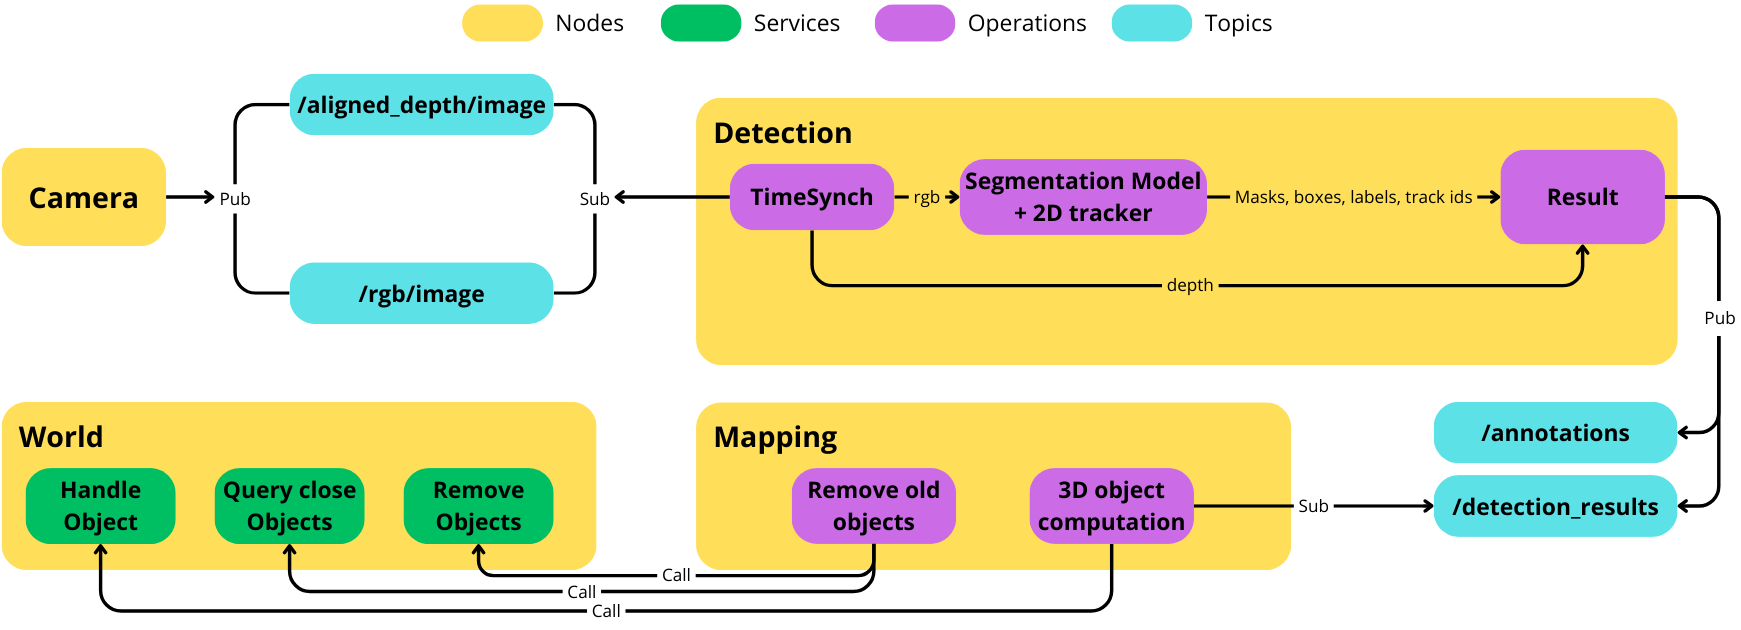
\includegraphics[width=1.0\textwidth]{figs/SW-struct.png}
    \caption{Software Structure}
    \label{fig:software_structure}
\end{figure}

\subsection[Detection Node]{Detection Node}
This node subscribes to the RGB and depth topics, performs instance segmentation, and publishes the results to the ROS network.
When RGB and depth images are published a callback function is triggered, this function acts a series of steps:
\subsubsection[YOLO]{YOLO - Instance Segmentation Model}
The YOLO model is used to perform instance segmentation, for further information about 
design choices and model details refer to section \ref{sec:instance_segmentation}.
This model has been implemented using the API provided by Ultralytics \cite{ultralytics_yolo_2023}.
In this application no batching is used since the model is running on a single image at a time.
This particular implementation offers also an implementation of the ByteTrack algorithm explained in section 
\ref{sec:byte_track} that allow to extract unique IDs for each detected object.
To call the YOLO model and the ByteTrack algorithm ultralytics api is called with the following code snippet:
\begin{python}
results = self.detector.track(
                frame,
                device=self.device,
                conf=DETECTION_CONFIDENCE,
                stream=True,
                persist=True,
                tracker=TRACKER,
                verbose=False,
            )
\end{python}
From the result, we extract segmentation masks, track IDs, prediction confidence scores, and class labels:
\begin{enumerate}
    \item \textbf{Class Labels}: These are the class labels of the detected objects, and they have shape \( n_{\text{pred}} \).
    \item \textbf{Segmentation Masks}: They are binary masks of shape \( n_{\text{pred}} \times h_{\text{img}} \times w\_{\text{width}} \) where at index \( [i, h, w] \) we have a 1 if pixel \( [h, w] \) belongs to pred \( i \) and 0 otherwise.
    \item \textbf{Track IDs}: They are unique IDs for each detected object, used to track objects across frames. They have shape \( n_{\text{pred}} \).
    \item \textbf{Prediction Confidence Scores}: These are the confidence scores of the model for each detected object, and they have shape \( n_{\text{pred}} \).
\end{enumerate}
From this step we do not consider 2D bounding boxes as 3D bounding boxes will be computed by from the objects point clouds.
<<<<<<< HEAD

\subsubsection[Detection Message]{Detection Message}
In order to publish the detection results to the ROS network, a custom message is defined.
This message is defined with the .msg extension and it is composed of the following fields:

\begin{python}
std_msgs/Header header #contains camera_frame_id and timestamp of the detection
# list of normalized xyxy points for each detection, need to be reshaped to (n, 4)
# to get the bounding boxes where n is len(labels)
int32[] boxes
int32[] ids
float32[] scores
# need to be reshaped to (n, h, w)
sensor_msgs/Image masks
sensor_msgs/Image depth
string[] labels
\end{python}

\subsection[Mapping Node]{Mapping Node}
This node functions as an intermediate node between the detection and world nodes. 
That because it contains informations about both the camera reference frame and the map reference frame.
It subscribes to the detection result topic and creates a 3D point cloud of the detected objects,
calls the services offered by the World node for:
\begin{itemize}
    \item Managing new detected objects
    \item Removing objects that are no longer present in the environment
\end{itemize}



\subsubsection[Mask Erosion]{Mask Erosion}
\noindent
\begin{minipage}{0.55\textwidth}
    From qualitative analysis, it was observed that the depth image produced by the camera had a particular type of artifact called depth bleeding as observed in Figure \ref{fig:depth_bleeding}.
    Depth bleeding is an artifact in depth imaging where the edges of objects appear larger than their actual size. 
    This occurs due to inaccuracies in the depth sensor, causing the contours of objects to “bleed” into surrounding areas.
    As a result, the depth image represents objects with exaggerated dimensions compared to the RGB image, 
    leading to imprecise depth measurements and distorted object boundaries.
\end{minipage}
\begin{minipage}{0.4\textwidth}
    \begin{figure}[H] % Using the figure environment to include in List of Figures
        \centering
        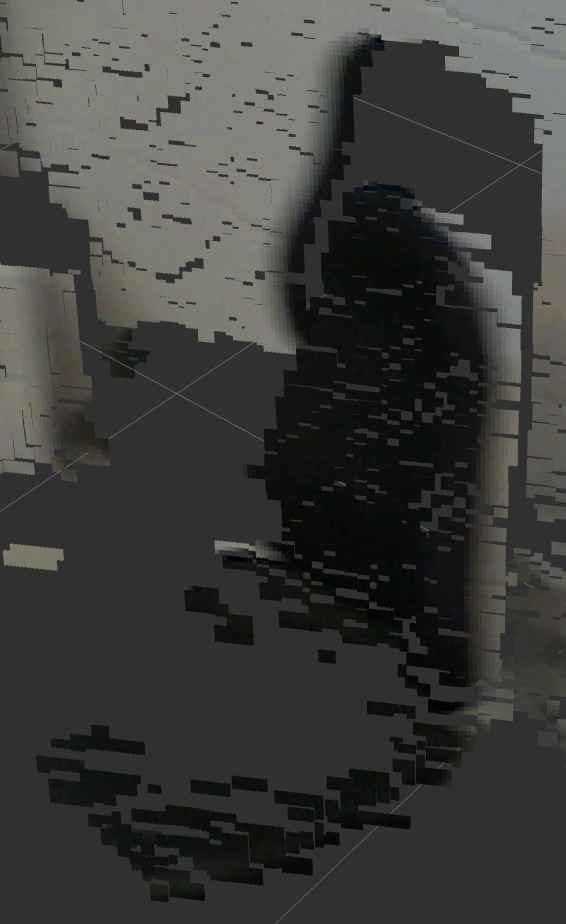
\includegraphics[width=\textwidth]{figs/depth_bleeding.png}
        \caption{Caption for Figure 1}
        \label{fig:figure1}
    \end{figure}
\end{minipage}
\hfill
\\Furthermore, the segmentation masks produced by the YOLO model are not perfect, and they often include pixels that do not belong to the object.
For this reason we apply a morphological operation called erosion to the segmentation masks.

\begin{table}[htbp]
    \centering
    \begin{tabular}{cc}
        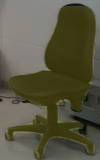
\includegraphics[width=0.25\textwidth]{figs/mask_no_erosion.png} & 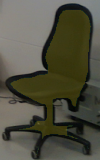
\includegraphics[width=0.25\textwidth]{figs/mask_erosion.png} \\
        \small Segmentation mask without erosion & \small Segmentation mask with erosion \\
        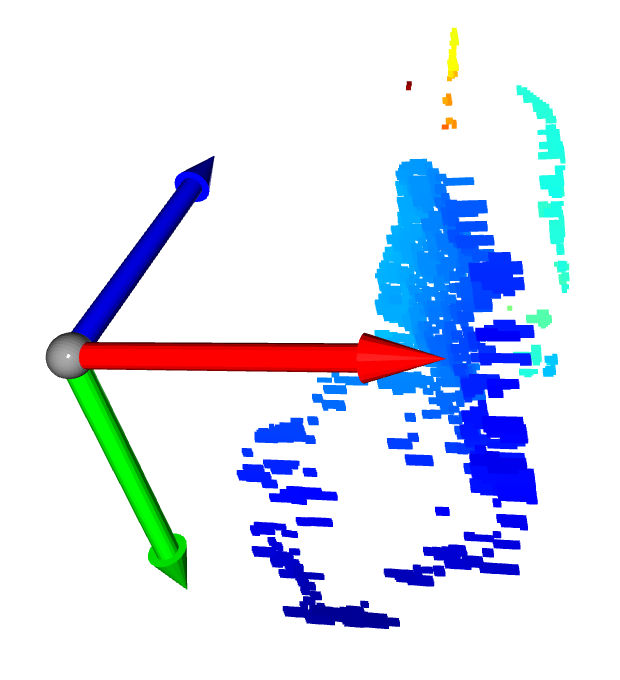
\includegraphics[width=0.25\textwidth]{figs/pc_no_erosion.png} & 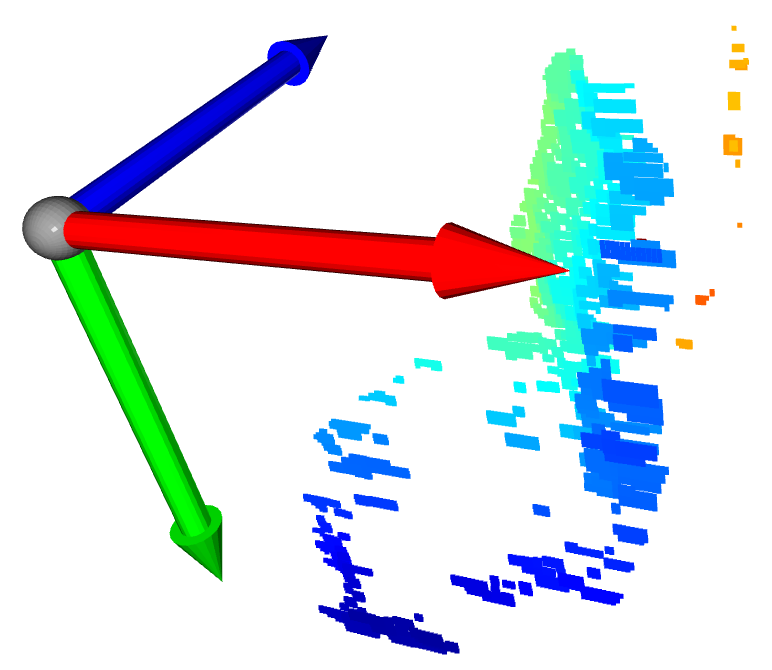
\includegraphics[width=0.25\textwidth]{figs/pc_erosion.png} \\
        \small Point cloud without mask erosion & \small Point cloud with mask erosion \\
    \end{tabular}
    \caption{Comparison between point clouds with and without mask erosion. Figure 1 and 2 show the segmentation masks before and after erosion. Figure 3 and 4 show the point clouds generated from the masks.}
    \label{fig:erosion_comparison}
\end{table}

\end{document}
=======
\subsection[Mask Erosion]{Mask Erosion}
Since depth acquired from this particular camera tends to ...
>>>>>>> cec88a7498d01c8161e2bd2d222022f28b949c03
